\documentclass[conference]{IEEEtran} % default font size: 10pt
\usepackage{times,microtype}

\usepackage{graphicx}
\usepackage[caption=false]{subfig}
\graphicspath{{images/}}

\usepackage{amsmath,amssymb,mathtools}

\renewcommand{\vec}[1]{\boldsymbol{#1}}
\DeclarePairedDelimiter{\abs}{\lvert}{\rvert}
\DeclarePairedDelimiter{\norm}{\lVert}{\rVert}

\usepackage{lipsum,xcolor} % TODO: remove once fully written

% numbers option provides compact numerical references in the text.
\usepackage[numbers]{natbib}
\usepackage{multicol}
\usepackage[bookmarks=true]{hyperref}

\pdfinfo{ % TODO: update info below
   /Author (Homer Simpson)
   /Title  (Robots: Our new overlords)
   % /CreationDate (D:20101201120000)
   /Subject (Robots)
   /Keywords (Robots;Overlords)
}

\begin{document}

% TODO: paper title
\title{Template paper for the \\Robotics: Science and Systems Conference}

% You will get a Paper-ID when submitting a pdf file to the conference system TODO: update info below
\author{Author Names Omitted. Paper-ID [add your ID here]}

%\author{\authorblockN{Michael Shell}
%\authorblockA{School of Electrical and\\Computer Engineering\\
%Georgia Institute of Technology\\
%Atlanta, Georgia 30332--0250\\
%Email: mshell@ece.gatech.edu}
%\and
%\authorblockN{Homer Simpson}
%\authorblockA{Twentieth Century Fox\\
%Springfield, USA\\
%Email: homer@thesimpsons.com}
%\and
%\authorblockN{James Kirk\\ and Montgomery Scott}
%\authorblockA{Starfleet Academy\\
%San Francisco, California 96678-2391\\
%Telephone: (800) 555--1212\\
%Fax: (888) 555--1212}}


% avoiding spaces at the end of the author lines is not a problem with
% conference papers because we don't use \thanks or \IEEEmembership


% for over three affiliations, or if they all won't fit within the width
% of the page, use this alternative format:
%
%\author{\authorblockN{Michael Shell\authorrefmark{1},
%Homer Simpson\authorrefmark{2},
%James Kirk\authorrefmark{3},
%Montgomery Scott\authorrefmark{3} and
%Eldon Tyrell\authorrefmark{4}}
%\authorblockA{\authorrefmark{1}School of Electrical and Computer Engineering\\
%Georgia Institute of Technology,
%Atlanta, Georgia 30332--0250\\ Email: mshell@ece.gatech.edu}
%\authorblockA{\authorrefmark{2}Twentieth Century Fox, Springfield, USA\\
%Email: homer@thesimpsons.com}
%\authorblockA{\authorrefmark{3}Starfleet Academy, San Francisco, California 96678-2391\\
%Telephone: (800) 555--1212, Fax: (888) 555--1212}
%\authorblockA{\authorrefmark{4}Tyrell Inc., 123 Replicant Street, Los Angeles, California 90210--4321}}


\maketitle

% ----------------------------------------------------------------------------------------

\begin{abstract}
MPC online control problem enhanced in CasADi, a framework written by \citet{Andersson2019}.
\end{abstract}

\IEEEpeerreviewmaketitle

\section{Introduction}

\textcolor{gray}{\lipsum[1]}

% ----------------------------------------------------------------------------------------

\section{Proposed approach} % TODO: if the method has a name, use it here as section title

\textcolor{gray}{\lipsum[2]}

\subsection{Vehicle model}

\textcolor{gray}{\lipsum[3]}

\subsection{Spatial formulation}

The race track, assumed planar, is modelled through the parametric 2D curve
\begin{equation}
\mathcal C(\alpha) = \{ \vec x (\alpha) = [x(\alpha), y(\alpha)]^T \in \mathbb{R}^2 : \alpha \in [\alpha_0, \alpha_f] \}
\end{equation}
%
that identifies the road centerline, and the 1D curve $\mathcal W(\alpha)$ that specifies the track width.
With reference to Figure~\ref{fig:scheme_frenet_serret_refsys}, the \emph{curve parameter} $\alpha$ uniquely selects a point $\vec F = \vec x(\alpha)$ that defines the origin of the \emph{Frenet-Serret frame} $\mathcal F = \{ \vec F, (\vec t, \vec p) \}$ whose unit vectors are, respectively, the tangent $\vec t$ and the normal $\vec p$ of the curve $\mathcal C$ in the point $\vec F$.
%
The vehicle reference system $\mathcal V = \{ \vec G, (\vec i, \vec j) \}$ can be expressed in terms of the moving frame $\mathcal F$ with a \emph{lateral displacement} $e_p$ along the track normal direction $\vec p$ and the \emph{heading error} $e_\psi$.
% = \psi_f - \psi_v
In order to maintain $\mathcal F$ side-by-side with $\mathcal V$, the Frenet-Serret system has to proceed together with the vehicle: this leads to a relation between vehicle and Frenet-Serret velocities that ultimately imposes a bound between time and $\alpha$ increments.

The final formulation of the vehicle model dynamics, % TODO: ref to standard formulation, if previously exposed
extended with lateral displacement, heading error and transposed in spatial domain is

\begin{equation} \left\{
\begin{aligned}
  u_{,\alpha} &= \frac{\norm{\hat{\vec x}_{,\alpha}}}{s_p} \left[ \frac{1}{m} (F_{x_1} - F_{y_1} \delta + F_{x_2} - X_a) + vr \right] \\
  v_{,\alpha} &= \frac{\norm{\hat{\vec x}_{,\alpha}}}{s_p} \left[ \frac{1}{m} (F_{x_1} \delta + F_{y_1} + F_{y_2}) - ur \right] \\
  r_{,\alpha} &= \frac{\norm{\hat{\vec x}_{,\alpha}}}{s_p} \left[ \frac{1}{I_{zz}} (F_{x_1} a_1 \delta + F_{y_1} a_1 - F_{y_2} a_2) \right] \\
  e_{p,\alpha} &= \frac{\norm{\hat{\vec x}_{,\alpha}}}{s_p} \left[ u \sin{e_\psi} + v \cos{e_\psi} \right] \\
  e_{\psi,\alpha} &= \norm{\hat{\vec x}_{,\alpha}} \left( \frac{r}{s_p} - k \right),
\end{aligned} \right.
\label{eq:vehicle_state_update_alpha_domain}
\end{equation}
%
where the notation $u_{,\alpha} = \frac{du}{d \alpha}$ has been used to shorten derivative notations.

\begin{figure}[htb] \centering
  \subfloat[]
    {\includegraphics[width=.5\linewidth]{example-image-a}} % NOTE: this needs `mwe' package
  \quad
  \subfloat[]{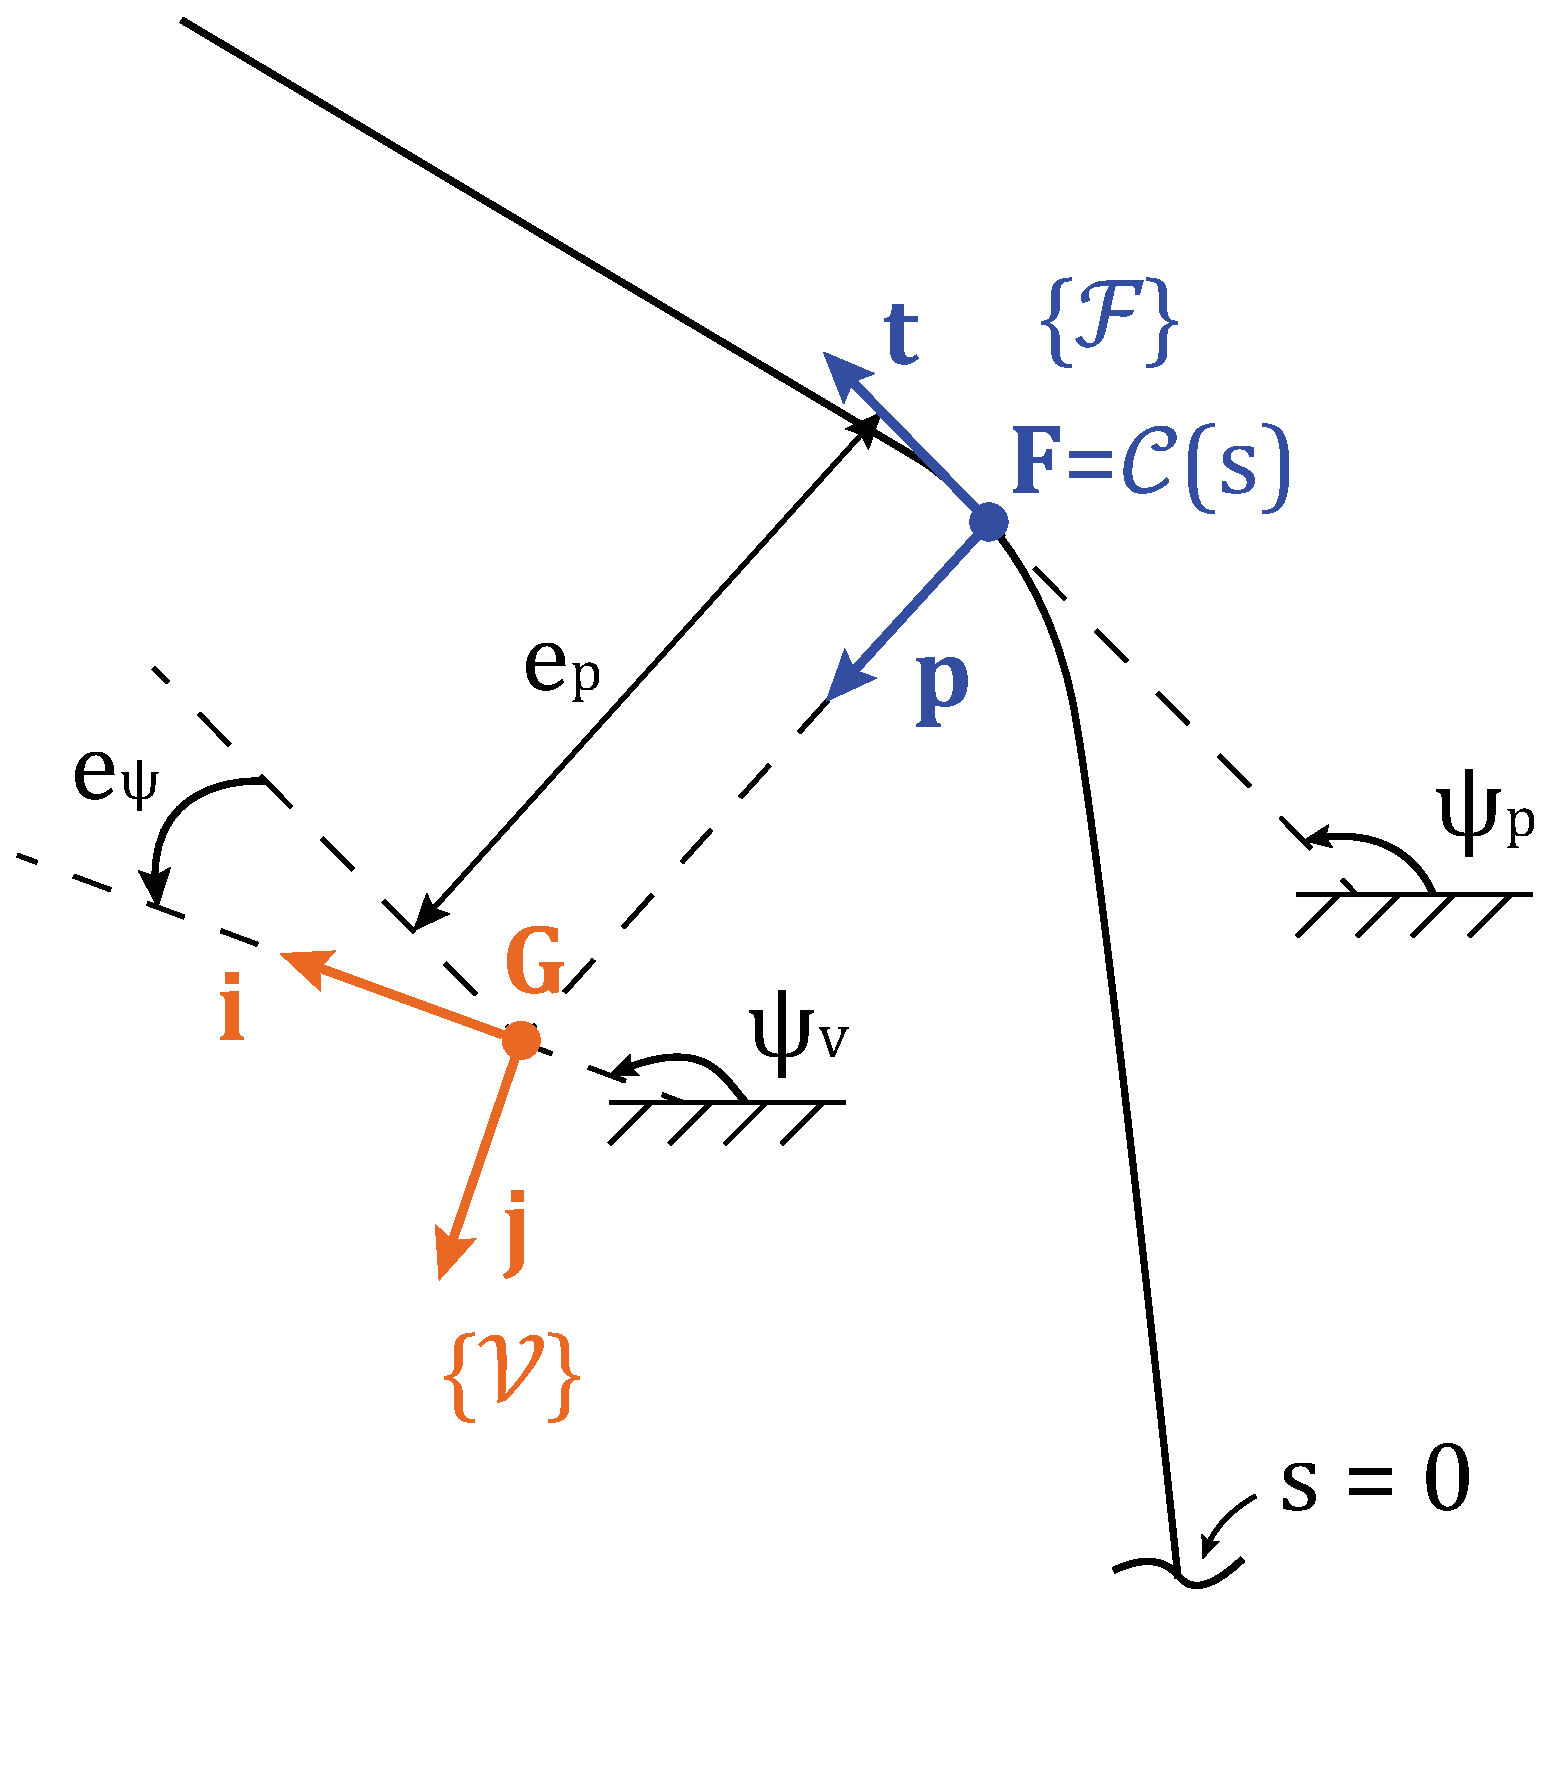
\includegraphics[width=.4\linewidth]{scheme_frenet_serret_refsys}
    \label{fig:scheme_frenet_serret_refsys}}
  \caption{(\textbf{a}) Something, maybe a vehicle model schematic; (\textbf{b}) vehicle pose respect to the Frenet-Serret reference system identified on the track curve.}
  \label{fig:scheme_frenet_serret}
\end{figure}

% \subsection{OCP problem formulation}

% The Optimal Control Problem (OCP) is

\subsection{Offset-free MPC}

\textcolor{gray}{\lipsum[4]}

% ----------------------------------------------------------------------------------------

\section{Preliminary results}

\textcolor{gray}{\lipsum[5]}

% ----------------------------------------------------------------------------------------

\section{Conclusion}
\label{sec:conclusion}

\textcolor{gray}{\lipsum[6]}

% ----------------------------------------------------------------------------------------

%% Use plainnat to work nicely with natbib.
\bibliographystyle{plainnat}
\bibliography{references}

\end{document} 